\documentclass{standalone}
\usepackage{tikz}
\usetikzlibrary{patterns, positioning}

\begin{document}
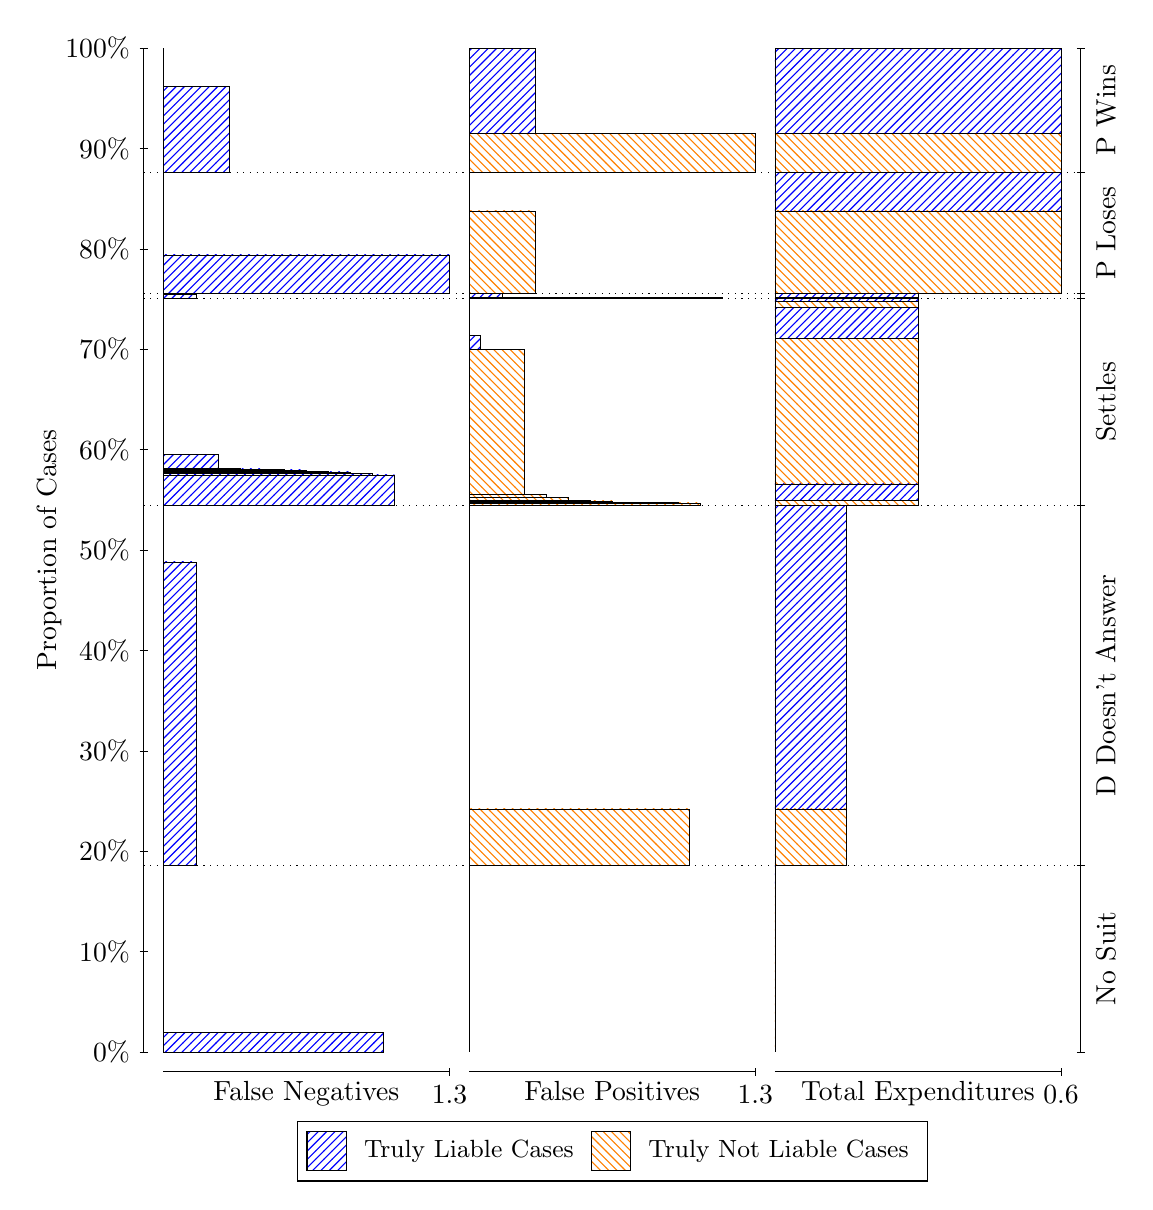
\begin{tikzpicture}
\draw[black, very thin] (1.5,1.75) -- (1.5,14.5);
\node[rotate=90, anchor=center] at (0.3, 8.125) {Proportion of Cases};
\draw[black, very thin] (1.45,1.75) -- (1.55,1.75);
\node[anchor=east] at (1.45, 1.75) {0\%};
\draw[black, very thin] (1.45,3.025) -- (1.55,3.025);
\node[anchor=east] at (1.45, 3.025) {10\%};
\draw[black, very thin] (1.45,4.3) -- (1.55,4.3);
\node[anchor=east] at (1.45, 4.3) {20\%};
\draw[black, very thin] (1.45,5.575) -- (1.55,5.575);
\node[anchor=east] at (1.45, 5.575) {30\%};
\draw[black, very thin] (1.45,6.85) -- (1.55,6.85);
\node[anchor=east] at (1.45, 6.85) {40\%};
\draw[black, very thin] (1.45,8.125) -- (1.55,8.125);
\node[anchor=east] at (1.45, 8.125) {50\%};
\draw[black, very thin] (1.45,9.4) -- (1.55,9.4);
\node[anchor=east] at (1.45, 9.4) {60\%};
\draw[black, very thin] (1.45,10.675) -- (1.55,10.675);
\node[anchor=east] at (1.45, 10.675) {70\%};
\draw[black, very thin] (1.45,11.95) -- (1.55,11.95);
\node[anchor=east] at (1.45, 11.95) {80\%};
\draw[black, very thin] (1.45,13.225) -- (1.55,13.225);
\node[anchor=east] at (1.45, 13.225) {90\%};
\draw[black, very thin] (1.45,14.5) -- (1.55,14.5);
\node[anchor=east] at (1.45, 14.5) {100\%};

\draw[black, very thin] (13.4,1.75) -- (13.4,14.5);
\draw[black, very thin] (13.35,1.75) -- (13.45,1.75);
\node[anchor=west] at (13.35, 1.75) {};
\draw[black, very thin] (13.35,4.1224) -- (13.45,4.1224);
\node[anchor=west] at (13.35, 4.1224) {};
\draw[black, very thin] (13.35,8.6876) -- (13.45,8.6876);
\node[anchor=west] at (13.35, 8.6876) {};
\draw[black, very thin] (13.35,11.324) -- (13.45,11.324);
\node[anchor=west] at (13.35, 11.324) {};
\draw[black, very thin] (13.35,11.383) -- (13.45,11.383);
\node[anchor=west] at (13.35, 11.383) {};
\draw[black, very thin] (13.35,12.922) -- (13.45,12.922);
\node[anchor=west] at (13.35, 12.922) {};
\draw[black, very thin] (13.35,14.5) -- (13.45,14.5);
\node[anchor=west] at (13.35, 14.5) {};

\draw[black, very thin, pattern color=blue, pattern=north east lines] (1.75,1.75) rectangle (4.5449,1.9996);
\draw[black, very thin, pattern color=orange, pattern=north west lines] (1.75,1.9996) rectangle (1.75,4.1224);
\draw[black, very thin, pattern color=blue, pattern=north east lines] (1.75,4.1224) rectangle (2.1692,7.9727);
\draw[black, very thin, pattern color=orange, pattern=north west lines] (1.75,7.9727) rectangle (1.75,8.6876);
\draw[black, very thin, pattern color=blue, pattern=north east lines] (1.75,8.6876) rectangle (4.6846,9.0797);
\draw[black, very thin, pattern color=blue, pattern=north east lines] (1.75,9.0797) rectangle (4.4051,9.0963);
\draw[black, very thin, pattern color=blue, pattern=north east lines] (1.75,9.0963) rectangle (4.1256,9.1181);
\draw[black, very thin, pattern color=blue, pattern=north east lines] (1.75,9.1181) rectangle (3.8462,9.122);
\draw[black, very thin, pattern color=blue, pattern=north east lines] (1.75,9.122) rectangle (3.5667,9.143);
\draw[black, very thin, pattern color=blue, pattern=north east lines] (1.75,9.143) rectangle (3.2872,9.1469);
\draw[black, very thin, pattern color=blue, pattern=north east lines] (1.75,9.1469) rectangle (3.0077,9.1563);
\draw[black, very thin, pattern color=blue, pattern=north east lines] (1.75,9.1563) rectangle (2.7282,9.1643);
\draw[black, very thin, pattern color=blue, pattern=north east lines] (1.75,9.1643) rectangle (2.4487,9.3352);
\draw[black, very thin, pattern color=orange, pattern=north west lines] (1.75,9.3352) rectangle (1.75,11.324);
\draw[black, very thin, pattern color=blue, pattern=north east lines] (1.75,11.324) rectangle (2.1692,11.373);
\draw[black, very thin, pattern color=orange, pattern=north west lines] (1.75,11.373) rectangle (1.75,11.383);
\draw[black, very thin, pattern color=blue, pattern=north east lines] (1.75,11.383) rectangle (5.3833,11.873);
\draw[black, very thin, pattern color=orange, pattern=north west lines] (1.75,11.873) rectangle (1.75,12.922);
\draw[black, very thin, pattern color=blue, pattern=north east lines] (1.75,12.922) rectangle (2.5885,14.01);
\draw[black, very thin, pattern color=orange, pattern=north west lines] (1.75,14.01) rectangle (1.75,14.5);
\draw[black, very thin, pattern color=orange, pattern=north west lines] (5.6333,1.75) rectangle (5.6333,3.8728);
\draw[black, very thin, pattern color=blue, pattern=north east lines] (5.6333,3.8728) rectangle (5.6333,4.1224);
\draw[black, very thin, pattern color=orange, pattern=north west lines] (5.6333,4.1224) rectangle (8.4282,4.8373);
\draw[black, very thin, pattern color=blue, pattern=north east lines] (5.6333,4.8373) rectangle (5.6333,8.6876);
\draw[black, very thin, pattern color=orange, pattern=north west lines] (5.6333,8.6876) rectangle (8.5679,8.7231);
\draw[black, very thin, pattern color=orange, pattern=north west lines] (5.6333,8.7231) rectangle (8.2885,8.726);
\draw[black, very thin, pattern color=orange, pattern=north west lines] (5.6333,8.726) rectangle (8.009,8.7292);
\draw[black, very thin, pattern color=orange, pattern=north west lines] (5.6333,8.7292) rectangle (7.7295,8.7303);
\draw[black, very thin, pattern color=orange, pattern=north west lines] (5.6333,8.7303) rectangle (7.45,8.7495);
\draw[black, very thin, pattern color=orange, pattern=north west lines] (5.6333,8.7495) rectangle (7.1705,8.7506);
\draw[black, very thin, pattern color=orange, pattern=north west lines] (5.6333,8.7506) rectangle (7.1705,8.7526);
\draw[black, very thin, pattern color=orange, pattern=north west lines] (5.6333,8.7526) rectangle (6.891,8.7958);
\draw[black, very thin, pattern color=orange, pattern=north west lines] (5.6333,8.7958) rectangle (6.6115,8.8302);
\draw[black, very thin, pattern color=orange, pattern=north west lines] (5.6333,8.8302) rectangle (6.3321,10.676);
\draw[black, very thin, pattern color=blue, pattern=north east lines] (5.6333,10.676) rectangle (5.7731,10.847);
\draw[black, very thin, pattern color=blue, pattern=north east lines] (5.6333,10.847) rectangle (5.6333,11.324);
\draw[black, very thin, pattern color=orange, pattern=north west lines] (5.6333,11.324) rectangle (8.8474,11.334);
\draw[black, very thin, pattern color=blue, pattern=north east lines] (5.6333,11.334) rectangle (6.0526,11.383);
\draw[black, very thin, pattern color=orange, pattern=north west lines] (5.6333,11.383) rectangle (6.4718,12.431);
\draw[black, very thin, pattern color=blue, pattern=north east lines] (5.6333,12.431) rectangle (5.6333,12.922);
\draw[black, very thin, pattern color=orange, pattern=north west lines] (5.6333,12.922) rectangle (9.2667,13.412);
\draw[black, very thin, pattern color=blue, pattern=north east lines] (5.6333,13.412) rectangle (6.4718,14.5);
\draw[black, very thin, pattern color=orange, pattern=north west lines] (9.5167,1.75) rectangle (9.5167,3.8728);
\draw[black, very thin, pattern color=blue, pattern=north east lines] (9.5167,3.8728) rectangle (9.5167,4.1224);
\draw[black, very thin, pattern color=orange, pattern=north west lines] (9.5167,4.1224) rectangle (10.425,4.8373);
\draw[black, very thin, pattern color=blue, pattern=north east lines] (9.5167,4.8373) rectangle (10.425,8.6876);
\draw[black, very thin, pattern color=orange, pattern=north west lines] (9.5167,8.6876) rectangle (11.333,8.7506);
\draw[black, very thin, pattern color=blue, pattern=north east lines] (9.5167,8.7506) rectangle (11.333,8.9657);
\draw[black, very thin, pattern color=orange, pattern=north west lines] (9.5167,8.9657) rectangle (11.333,10.811);
\draw[black, very thin, pattern color=blue, pattern=north east lines] (9.5167,10.811) rectangle (11.333,11.203);
\draw[black, very thin, pattern color=orange, pattern=north west lines] (9.5167,11.203) rectangle (11.333,11.283);
\draw[black, very thin, pattern color=blue, pattern=north east lines] (9.5167,11.283) rectangle (11.333,11.324);
\draw[black, very thin, pattern color=orange, pattern=north west lines] (9.5167,11.324) rectangle (11.333,11.334);
\draw[black, very thin, pattern color=blue, pattern=north east lines] (9.5167,11.334) rectangle (11.333,11.383);
\draw[black, very thin, pattern color=orange, pattern=north west lines] (9.5167,11.383) rectangle (13.15,12.431);
\draw[black, very thin, pattern color=blue, pattern=north east lines] (9.5167,12.431) rectangle (13.15,12.922);
\draw[black, very thin, pattern color=orange, pattern=north west lines] (9.5167,12.922) rectangle (13.15,13.412);
\draw[black, very thin, pattern color=blue, pattern=north east lines] (9.5167,13.412) rectangle (13.15,14.5);
\draw[black, dotted] (1.5,4.1224) -- (13.4,4.1224);
\draw[black, dotted] (1.5,8.6876) -- (13.4,8.6876);
\draw[black, dotted] (1.5,11.324) -- (13.4,11.324);
\draw[black, dotted] (1.5,11.383) -- (13.4,11.383);
\draw[black, dotted] (1.5,12.922) -- (13.4,12.922);
\draw[black, very thin] (1.75,1.5) -- (5.3833,1.5);
\node[anchor=north] at (3.5667, 1.5) {False Negatives};
\draw[black, very thin] (5.3833,1.45) -- (5.3833,1.55);
\node[anchor=north] at (5.3833, 1.45) {1.3};

\draw[black, very thin] (5.6333,1.5) -- (9.2667,1.5);
\node[anchor=north] at (7.45, 1.5) {False Positives};
\draw[black, very thin] (9.2667,1.45) -- (9.2667,1.55);
\node[anchor=north] at (9.2667, 1.45) {1.3};

\draw[black, very thin] (9.5167,1.5) -- (13.15,1.5);
\node[anchor=north] at (11.333, 1.5) {Total Expenditures};
\draw[black, very thin] (13.15,1.45) -- (13.15,1.55);
\node[anchor=north] at (13.15, 1.45) {0.6};

\node[black, centered, rotate=90] at (13.72, 2.9362) {No Suit};
\node[black, centered, rotate=90] at (13.72, 6.405) {D Doesn't Answer};
\node[black, centered, rotate=90] at (13.72, 10.006) {Settles};

\node[black, centered, rotate=90] at (13.72, 12.152) {P Loses};
\node[black, centered, rotate=90] at (13.72, 13.711) {P Wins};

\draw (7.449999999999999,1.5) node[draw=none] (baseCoordinate) {};
\begin{scope}[align=center]
        \matrix[scale=0.5, draw=black, below=0.5cm of baseCoordinate, nodes={draw}, column sep=0.1cm]{
            \node[rectangle, draw, minimum width=0.5cm, minimum height=0.5cm, pattern=north east lines, pattern color=blue] {}; &
            \node[draw=none, font=\small] (B) {Truly Liable Cases}; &
            \node[rectangle, draw, minimum width=0.5cm, minimum height=0.5cm, pattern=north west lines, pattern color=orange] {}; &
            \node[draw=none, font=\small] (B) {Truly Not Liable Cases}; \\
            };
\end{scope}

\end{tikzpicture}
\end{document}